%READ THROUGH AND ACCEPTED BY: CHRIS, 23-05-2017 (NO COMPILE)
\chapter{Performance Analysis}
\label{ch:perf_analy}

In this chapter, the performance of each concept is analysed and a trade-off is performed. First, in \autoref{sec:trade_perf}, a summary trade-off table of the whole chapter is illustrated. Then a preliminary mass estimation of each concept is performed in \autoref{sec:mass_esti}, followed by a determination of the geometric properties in \autoref{sec:geom_prop}. Then, the endurance and range properties are analysed in \autoref{sec:endu_ana} and \autoref{sec:range_ana} and finally in \autoref{sec:power_ana} the required power for each concept is calculated. For the different concepts, the used mass estimation methods are not always the same. This has to do with the different available data. 

\section{Performance Trade-Off}
\label{sec:trade_perf}

This section illustrates the final trade-off of the performance analysis. First, a brief summary is shown in \autoref{tab:perform_trade} and then the grading system used for the trade-off is explained.
\subsection{Summary}
\label{sec:perf_sum}

In this section, the final performance trade-off is illustrated in \autoref{tab:perform_trade}. It can be seen, that The Winged Quadcopter and The Prandtl Box score best in terms of performance. This mainly comes from their low mass estimations and higher aspect ratio analysis. Then The Tandem and The Tiltrotor score worst on performance properties. Both of them are complex design which require a high mass in order to attain the required performance set by the stakeholders. 

\begin{table}[H]
    \centering
    \caption{Performance Sub Trade-Off}
    \label{tab:perform_trade} 
    \begin{tabular}{r|>{\centering}p{2.5cm}:>{\centering}p{2.5cm}:>{\centering}p{2.5cm}|c} 
    \textbf{Concept \rotatebox{90}{\hspace{0.5cm}Criterion}}    & 
    \rotatebox{90}{\textbf{Endurance}}                      &
    \rotatebox{90}{\textbf{Range}}                           & 
    \rotatebox{90}{\textbf{Required Power}}                          & 
    \rotatebox{90}{\textbf{Cumulative}}                       
    \\ \midrule
    Tailsitter      & - & 0 & + & 50\% 
    \\\hdashline
    Tandem          & - & - & \texttt{-{}-} & 17\% 
    \\\hdashline
    Prandtl Box     & ++ & + & - & 66.5\% 
    \\\hdashline
    Tiltrotor       & \texttt{-{}-} &  \texttt{-{}-} &  0 & 17\% 
    \\\hdashline
    Winged Quad.    & + & + & ++ & 83\% 
    \\ \midrule\midrule
    Weight          & 0.33  & 0.33  & 0.33  &  
    \end{tabular}
\end{table}

\subsection{Grading System}
\label{sec:grading_sys_perf}

The whole performance chapter uses numerical values in order to obtain trade-off results. As it is not possible yet to accurately generate results due to a lack of battery information and other relevant data, a valid grading system has to be obtained. For this, first the average of all of the values is calculated. Then, the percentage of each value towards the average is used as grading system. The grading system in \autoref{tab:grad_perf} is used. 

\begin{table}[htb]
\centering
\caption{Performance Grading System}
\label{tab:grad_perf}
    \begin{tabular}{ll}
    \toprule
    \textbf{Rating} & \textbf{Percentage of average} \\
    \midrule
    ++ &  more than 130\% of average\\\hdashline
    +  & 110\% up to and including 130\% of average\\\hdashline
    0  & 90\% up to and including 110 \% of average\\\hdashline
    -  & 70\% up to and including 90\% of average\\\hdashline
    \texttt{-{}-}& less than 70\% of average\\
    \bottomrule
    \end{tabular}
\end{table}

\label{sec:perf_appr}

%This chapter did not ahear to the standard structure, is it possible to change it to fit it that way?
% X Ground Handling
% X.1 Trade-Off
% X.1.1 Summary
% X.1.2 Grading System
% X.2 Criteria
% X.2.1 Criteria #1 < explain a bit how it influences
% etc
% X.2.X Criteria Weights
% X.3 Concept Analysis
% X.3.1 Concept 1 < here you explain how much + or - each concept gets for each criteria
% etc

\section{Mass Estimation}
\label{sec:mass_esti}

For the mass estimation, statistical analysis is performed; by means of collecting reference aircraft, the take-off mass estimation for the UAV concepts are obtained. 

Unfortunately, for some concepts no data could be found with comparable performance. In these cases, it has been chosen to use UAVs from a different mass category. By means of finding the $\frac{M_{payload}}{M_{TO}}$ ratio and by taking into account the 10kg payload capacity requirement, a UAV take-off mass estimation can be obtained.

In other words, the payload capacity is scaled according to the payload capacity of 10kg as set in the requirements. In this way an estimated take-off mass is found for the specific configurations that should have the right payload capacity.

\subsection{The Tailsitter}
The Tailsitter concept is based on a flying wing using a rotor on its nose as propulsion system. \autoref{tab:flyingwing} shows the payload and take-off mass of similar UAVs: the Atmos\footnote{\url{http://www.atmosuav.com/}, Accessed 12-05-2017}, the Firefly 6 \footnote{\url{https://www.birdseyeview.aero/}, Accessed 15-05-2017}, the Fury 1500 \footnote{\url{http://www.airforce-technology.com/projects/fury-1500-uav/}, Accessed 12-05-2017} and the Cantas E \footnote{\url{http://newspacetechnologies.cz/cantas-uas-project/}, Accessed 22-05-2017}. It also shows their respective ratio. The average of the ratios is used to calculate a the payload over take-off ratio for The Tailsitter. With this ratio it is possible to calculate the mass.

\begin{table}[htb]
    \centering
    \caption{Flying Wing Reference Aircraft}
    \label{tab:flyingwing}
    \begin{tabularx}{\textwidth}{lccc}
        \toprule
        \textbf{Reference drone}    & \textbf{Payload Mass [kg]}     & \textbf{MTOW [kg]}      & \textbf{Payload/Take-Off ratio}          \\\midrule
        Atmos                       & 0.8                            & 4.5                     & 5.63  \\\hdashline
        Firefly 6                   & 0.7                            & 4.1                     & 5.86 \\\hdashline
        Cantas E                    & 10                             & 65                      & 6.5     \\\hdashline             
        Fury 1500                   & 34                             & 136                     & 4 \\\midrule
        Average                     &                                &                         & 5.49 \\\bottomrule
    \end{tabularx}
\end{table}

The UAV should be able to carry a payload of at least 10 kg, this gives a mass of approximately 55 kg for the Tailsitter concept. 

\subsection{The Tandem}
%written by Bryan and Piotr

 In order to estimate the mass of The Tandem, two reference UAVs are chosen. The first one is the DHL Parcelcopter that has one rotating wing\footnote{\url{http://www.dhl.com/en/press/releases/releases_2016/all/parcel_ecommerce/successful_trial_integration_dhl_parcelcopter_logistics_chain.html}, Accessed 15-05-2017}. 
 
\begin{comment}
\begin{figure}[H]
    \centering
    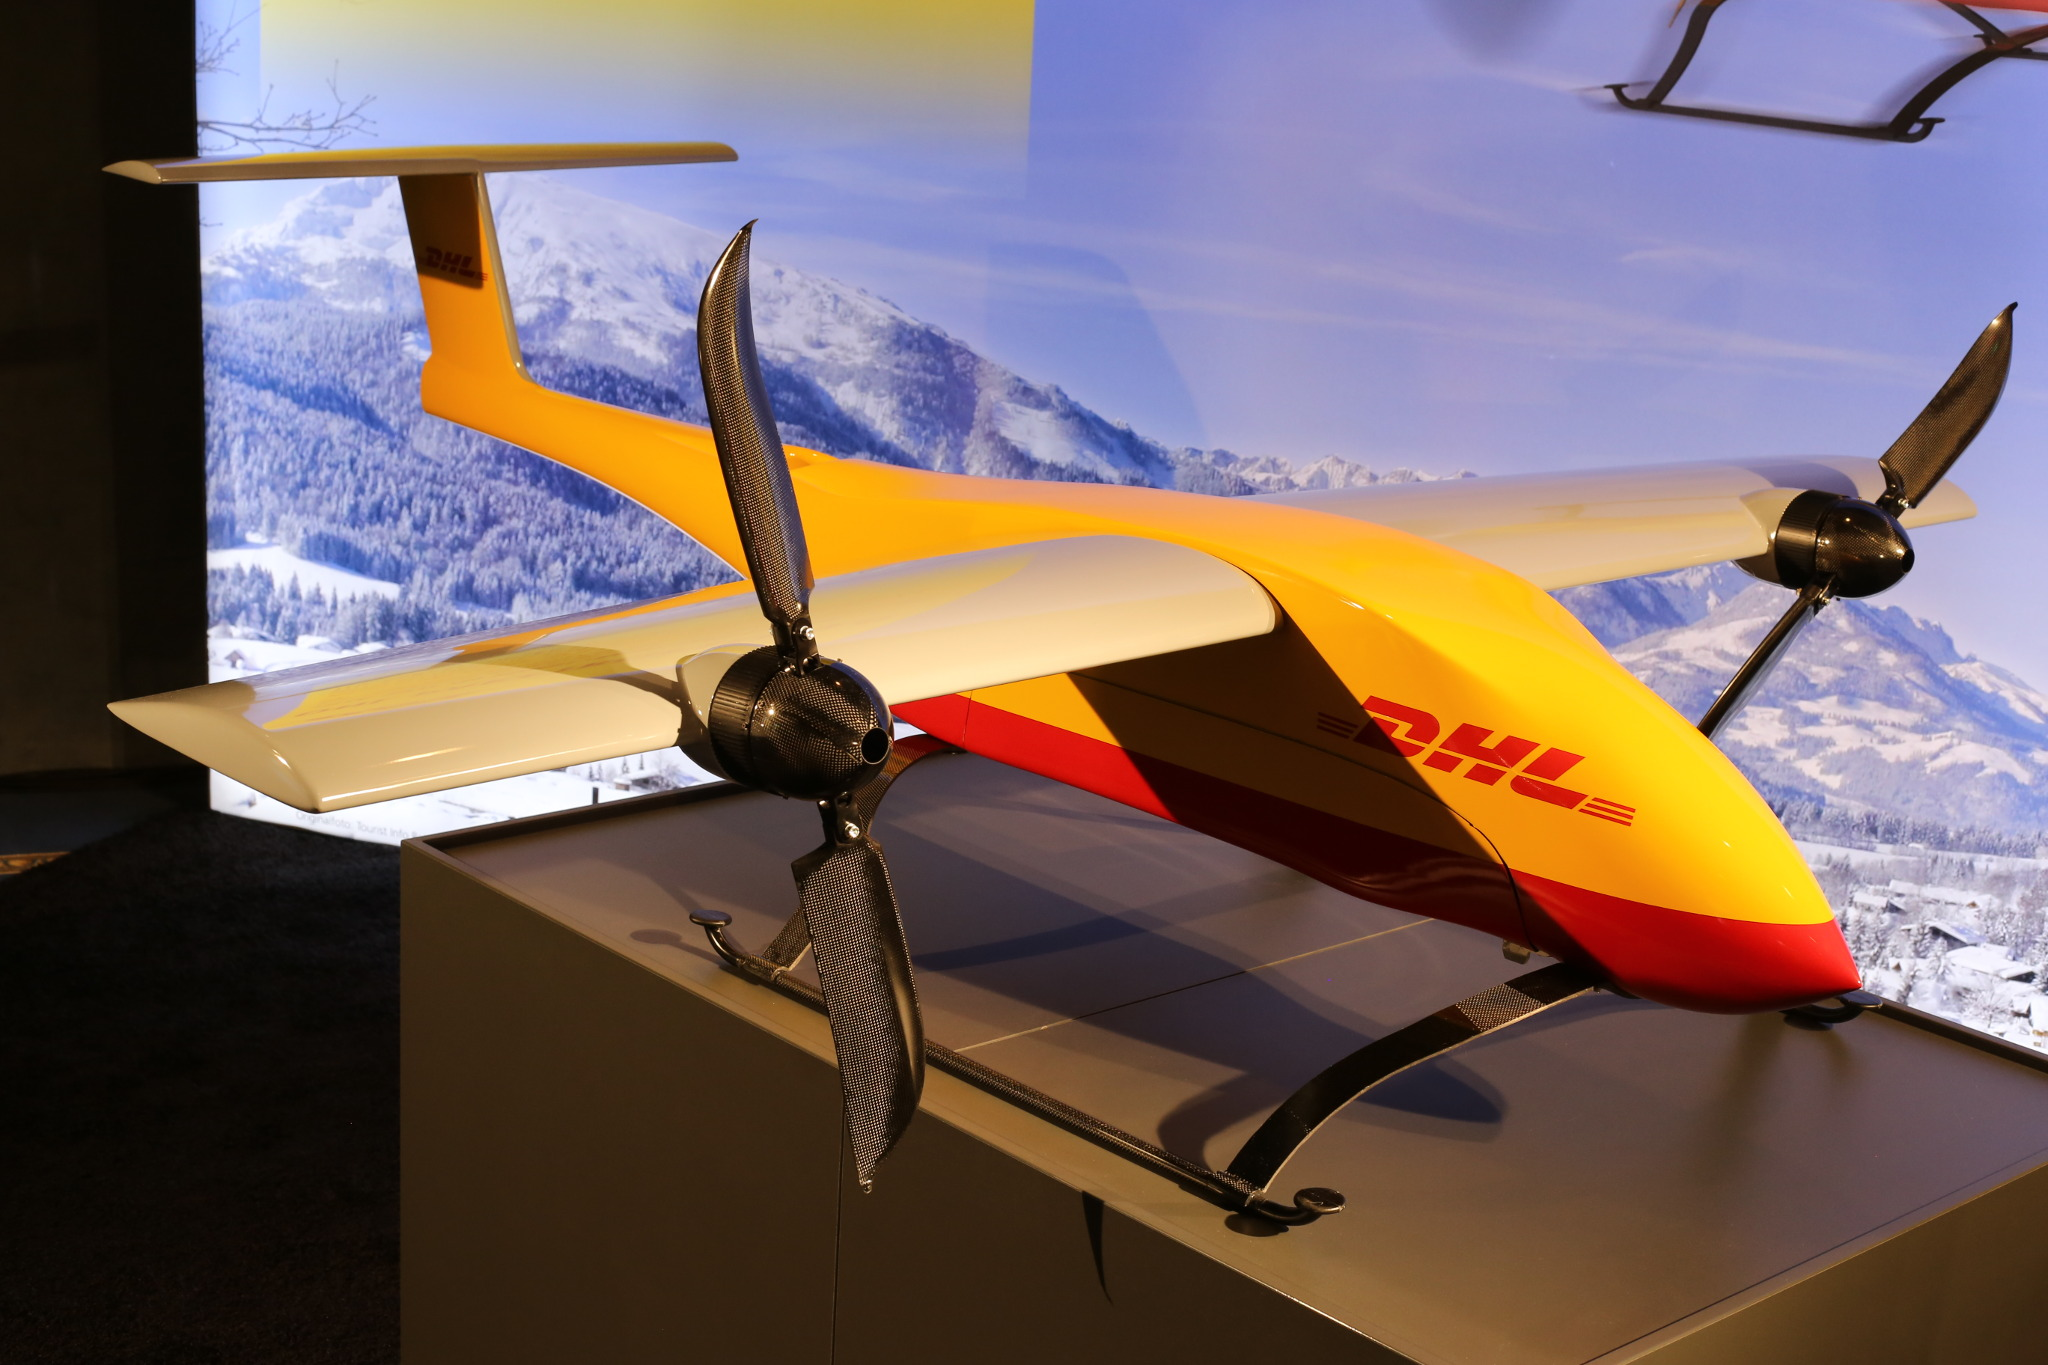
\includegraphics[width=0.6\textwidth]{PerformanceAnalysis/Figures/DHLparcelcopter3.jpeg}
    \caption{DHL Parcelcopter 3.0}
    \label{fig:parcelcopter}
\end{figure}
\end{comment}

The Maximum Take-Off Weight (MTOW) for this UAV is 14 kg, and the corresponding maximum payload mass is 2 kg. Since The Tandem has two rotating wings, additional mass has to be added to Parcelcopter in order to compensate for having only one wing. The structural mass of the wing is approximated to be 10\% of MTOW \cite{uav_weight}, thus having two rotating wings will result in a MTOW increase of 1.4 kg. With MTOW of 15.4 kg and payload of 2 kg, a scaling factor of 5 is applied such that the UAV meets the required payload mass of 10 kg. 

The resulting MTOW of The Tandem is 77 kg, yet it must be noted that The Tandem has no empennage, and intrinsically has a smaller wingspan than the reference aircraft, since the wing surface area can be divided amongst two wings. Both of these factors each reduce the MTOW by 5\% each\cite{uav_weight}. Therefore, the MTOW of The Tandem becomes 70 kg based on an analysis using Parcelcopter. 

The other reference UAV is developed by Chiba University\footnote{\url{http://www.barnardmicrosystems.com/UAV/milestones/tilt_wing.html}, Accessed 22-05-2017}. it has payload mass of 5 kg and MTOW of 23 kg. In order to meet the required payload mass of 10 kg, a scaling factor of 2 is applied. The UAV will have MTOW of 46 kg and payload mass of 10 kg. Due to lack of reference UAVs, data for two reference UAVs is combined in order to carry out a robust analysis. Thus, an average of MTOW is taken. The MTOW of The Tandem is determined to be 58 kg.

\begin{comment}
\begin{figure}[H]
    \centering
    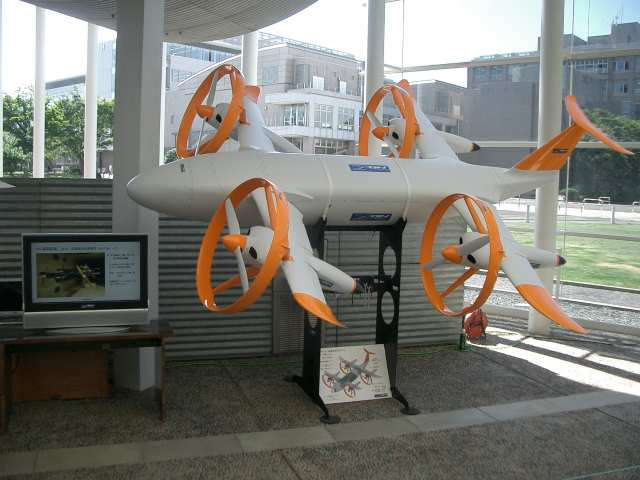
\includegraphics[width=0.6\textwidth]{PerformanceAnalysis/Figures/japtandem.jpg}
    \caption{Chiva University Tandem UAV}
    \label{fig:japtandem}
\end{figure}
\end{comment}
\subsection{The Prandtl Box}

The mass estimation for The Prandtl Box design is based on a comparable design proposed by AVY\footnote{\url{http://www.avy.eu/}, Accessed 12-05-2017}. This design has, with regard to the specifications and performance, much resemblance with the requirements set for this design. The mass of the AVY hybrid UAV can thus be considered as a reliable estimate for this design concept.

AVY claims that the Manufacturer's Empty Weight (MEW) is 13 kg. Based on a definition of MEW, it does not include mass of a battery and payload. By rearranging \autoref{eq:range} and \autoref{eq:endurance}, which can be found in \cref{sec:range_ana,sec:endu_ana}, a preliminary mass of the battery is determined to be 15 kg in order to obtain a range of 200 km and minimum endurance of 1 hour for a conventional-type UAV. With the required payload of 10 kg, the MTOW of The Prandtl Box becomes 38 kg. 

\subsection{The Tiltrotor Concept}
For the mass evaluation of this concept, the mass sensitive components have to be identified. The main component to be considered is the tilting rotor at the wingtips. This component will contribute significantly to the mass of the design. The main reason for this is the fact that the rotatable engines on the wing tips will need strong structural support to counter the strong forces and bending moments it introduces.

%The main reason for this is the fact that these rotating mechanisms have a high level of complexity, this results in an increase of mass. Besides this, there are structural reasons as well; due to the mounting of these complex mechanism at the wing tips, extra structural support is required. Furthermore, the introduction of loads at the wingtips by the engines require more structural support as well. All this extra required structural support will add to the total structural mass of the design.

For the mass estimation the data of three UAVs is consulted. In \autoref{tab:Tilt} the values are documented. By comparing the payload mass over take-off mass ratios of the reference vehicles. The used reference UAVs in this analysis are the Kari TR-60\footnote{\url{http://www.janes.com/article/63543/dx-korea-2016-kari-unveils-tr60-tiltrotor-uav}, Accessed 12-05-2017}, the Bell Eagle Eye\footnote{\url{https://fas.org/irp/program/collect/eagle-eye.htm}, Accessed 12-05-2017} and the Vertex VTOL UAS\footnote{\url{http://www.comquestventures.com/vertex-vtol-uas/\#imageclose-866},  Accessed 12-05-2017}. The Kari TR-60 together with the Vertex VTOL UAS is, with regard to performance, relatively close to the design parameters. The Bell Eagle Eye, however, deviates significantly in performance. This might explain the higher Take-Off/Payload Mass ratio. That is why the Bell Eagle Eye is regarded as an outlier with its ratio of 11.3. The disregarded vehicle is indicated with a asterisk in the table.  

%%Also two manned tiltrotor air vehicles are considered, namely the V-22 Osprey\footnote{\url{http://www.boeing.com/defense/v-22-osprey/}, Accessed 12-05-2017} and the AgustaWestland AW609\footnote{\url{https://web.archive.org/web/20100606090212/http://www.agustawestland.com/product/ba609}, Accessed 12-05-2017}. However manned air vehicles  will be ignored in this mass estimation. This is done for the reason that these vehicles do not really belong in the same vehicle category. Although these vehicles also use the Tiltrotor concept, \autoref{tab:Tilt} shows a big differences in values for the ratios. The table shows that the payload mass over take-off mass ratio differs significantly from the ratio of the UAVs (difference between approximately 7 for UAVS and 2-3 for manned vehicles). This can be explained if these manned air vehicles are further considered. The list of specifications shows no resemblance with the required performance specifications of this design. 



\begin{table}[h]
\centering
\caption{Tiltrotor Reference Aircraft}
\label{tab:Tilt}
    \begin{tabular}{lccc}
        \toprule
        \textbf{Reference UAV}   & \textbf{Payload Mass [kg]} & \textbf{MTOW [kg]} & \textbf{Take-off/Payload Ratio} \\\midrule
        Vertex VTOL UAS & 0.7               & 4.3       & 6.14               \\\hdashline
        Kari TR-60      & 30                & 210       & 7                  \\\hdashline
        Bell Eagle Eye*  & 90                & 1020      & 11.3               \\\midrule
        Average         &                   &           & 6.57                   \\\bottomrule
    \end{tabular}
\end{table}

With the average payload mass over take-off mass ratio it is possible to compute the MTOW for The Tiltrotor. The MTOW estimation for The Tiltrotor is approximately 66kg.

%Maybe state  that the references show that specifications of the reference A/C in a schematic way. They will not be mentioned in the report.

\subsection{The Winged Quadcopter}
The Winged Quadcopter is the most common configuration chosen for the design of a Hybrid UAV. As a result, there is quite a large number of reference UAVs that reveal useful trends when trying to get an initial mass estimate of The Winged Quadcopter. Comparing the payload weights of the various reference UAVs to their maximum take-off weight (MTOW) allows one to estimate the MTOW of this concept based on its required payload mass. Using ten reference Hybrid UAVs, the relationship between the payload weight and the MTOW can be established. This relationship is shown in \autoref{fig:perfthing}.


\begin{figure}[H]
\label{fig:perfthing}
\centering
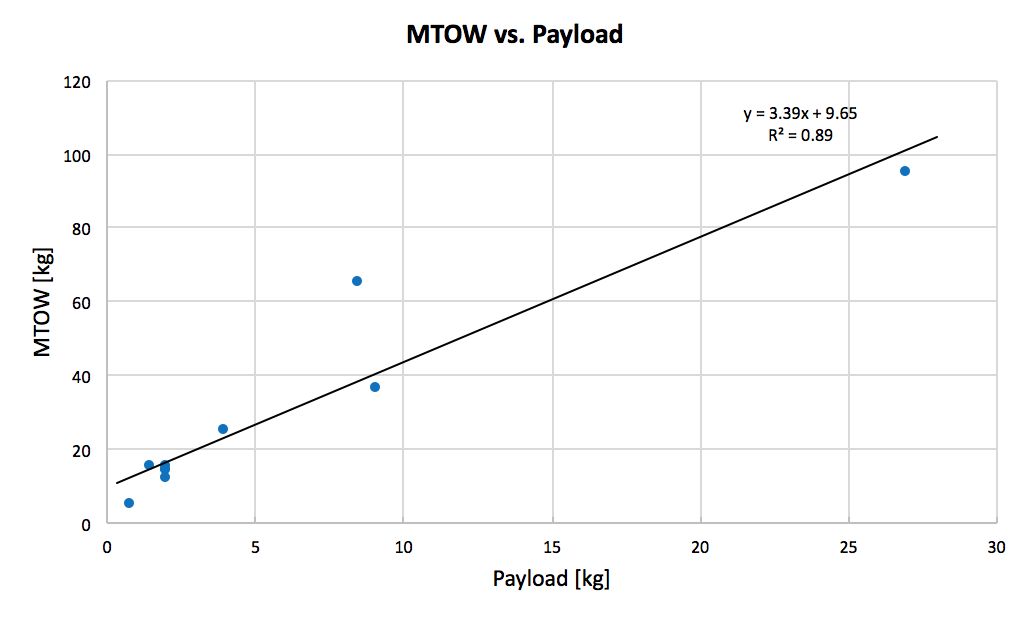
\includegraphics[width = 0.75\textwidth]{PerformanceAnalysis/Figures/MTOW_vs_PL_WQ.png}
\caption{Graph of MTOW vs. Payload Mass}
\end{figure}

The references can be found in \autoref{sec:refvoorgev}. From the graph, a linear relationship between MTOW and payload mass can be identified. The R$^2$ of this trend line is approximately 0.89, signifying a sufficiently good fit. Using the equation of the trend line, a payload mass of 10 kg results in an estimated MTOW of 44 kg.

\subsection{Summary of Mass Estimation}
The estimated MTOWs were all developed based on reference aircraft by comparing the MTOWs to the payloads carried. The MTOWs of the five concepts capable of carrying a payload of 10 kg are summarised in \autoref{tab:mass_summ}. 

\begin{table}[htb]
\centering
\caption{Table of Mass Estimates for Each Concept}
\label{tab:mass_summ}
    \begin{tabular}{lc}
        \toprule
            \textbf{Concept}           & \textbf{MTOW [kg]}\\ \midrule
         The Tailsitter       & 55 \\ \hdashline
         The Tandem           & 58 \\ \hdashline
         The Prandtl-Box      & 38   \\ \hdashline
         The Tiltrotor        & 66 \\ \hdashline
         The Winged Quad.     & 44 \\ \bottomrule
    \end{tabular}
\end{table}

\section{Geometric Properties}
\label{sec:geom_prop}

For the further analysis of the different designs, a preliminary estimation of the geometric properties is required, namely the Aspect Ratio (AR), the Oswald factor (e), and the zero-lift drag coefficient ($C_{D_{0}}$). Where possible, the parameters are roughly estimated from the sketches created in \autoref{ch:concepts}. Although more reliable values are needed for later stages of the design phase, initial estimations are adequate for relative comparisons between the five concepts. 

\subsection{Aspect Ratio}
\label{sec:aspe_rati}

The aspect ratio of each concept has to be estimated in order to perform a preliminary performance analysis. As most of the dimensional properties of the concepts are not known yet at this stage of the design, a preliminary aspect ratio estimation is performed using the sketches created in \autoref{ch:concepts} and in the previous report \cite{baseline}.

Starting with The Winged Quadcopter, an AR of 8 is approximated based on visual inspection of the preliminary sketch.
For the tilt-rotor concept, an aspect ratio of 5.5 is obtained by inspection. This value is also verified by comparing it to the V-22 aspect ratio.
For The Tandem, inspecting the preliminary sketches gives a final aspect ratio of 6.5. The smaller aspect ratio comes from the fact that two wings are used for the production of lift instead of one. As they need around the same amount of surface area, the wingspan can decrease and hence it has a smaller aspect ratio. Using the same reasoning, The Prandtl Box would also receive an aspect ratio of 6.5. However, the vertical wing segments are also included in the calculations of the wingspan and hence The Prandtl Box will receive an aspect ratio of 7.
Finally, The Tailsitter uses nearly its whole surface area for lift, hence a low wingspan is required. This will reduce the aspect ratio considerably. From the sketch in \autoref{ch:concepts} an AR of 4.5 is estimated for The Tailsitter. \autoref{tab:AR} gives an overview of the used aspect ratios for the performance trade-off.

\begin{table}[htb]
    \centering
    \caption{Preliminary Aspect Ratios for All Concepts}
    \label{tab:AR}
    \begin{tabularx}{0.5\textwidth}{lc}
        \toprule
        \textbf{Concept} & \textbf{Aspect Ratio [-]} \\
        \midrule
        The Tailsitter          & 4.5 \\ \hdashline
        The Tandem              & 6.5 \\ \hdashline
        The Prandtl Box         & 7  \\ \hdashline
        The Tiltrotor           & 5.5   \\ \hdashline
        The Winged Quad.        & 8 \\\bottomrule
    \end{tabularx}
\end{table}

\subsection{Oswald Factor}

With exception of The Prandtl Box concept, the Oswald factor of all the concepts is taken to be equal to 0.8, which is the typical value for remote controlled model aircraft \cite{drag_ch3}. The variation of the Oswald factor between the four concepts is small ($\pm$5\%), thus it will have a negligible influence on the change in performance per concept. In addition, the errors caused by the assumptions in the other estimations will most likely be greater than the contribution of the Oswald factor to the change in performance, more so enforcing a constant Oswald factor.

For the Prandtl wing box however, the Oswald factor will be significantly different. According to a Stanford research paper on non-planar wings \cite{Oswald}, the Oswald factor can be estimated to be 1.31. A Prandtl box has a quasi-closed C-wing structure, that includes small vertical wing segments. The dimension of the vertical wing segment strongly influences the Oswald efficiency factor; the greater this segment, the higher the Oswald factor. However, our concept will have a limited vertical wing segment. That is why the corresponding Oswald efficiency factor will have a value of 1.31. 

\subsection{Zero-Lift Drag Coefficient}
\label{sec:zeroliftdrag}

The zero-lift drag coefficient ($C_{D_{0}}$) originates from parasitic drag mainly dependent on the geometry of an aircraft. Therefore, in order to estimate $C_{D_{0}}$ it is sensible to divide an aircraft into geometrical groups making it possible to analyse the different concepts in a structured manner. In this analysis the concepts are divided into fuselage, wing and tail groups.

The analysis consists of determining the amount of fuselages, wings and tails for each concept based on the sketches shown in \autoref{sec:chosconc}. A reference UAV is considered first, which comprises one fuselage, one pair of wings, and one tail. All concepts are compared to this reference UAV.

The Tailsitter concept has no fuselage (it is incorporated into the main wing), one pair of wings, and half a tail, since it only has a vertical fin. The horizontal fin is already incorporated into the main wing, hence the contribution of the tail to the parasitic drag is halved. The Tandem concept has one fuselage, two pairs of wings and no tail. The Prandtl Box concept has one fuselage, two pairs of wings and again only half a tail for the same reason as the Tailsitter concept. The Tiltrotor and Winged Quadcopter concepts each have one fuselage, one pair of wings and one tail. Therefore their configuration is considered identical to the reference aircraft in this analysis.

The contribution of the fuselage, wing and tail groups to the $C_{D_{0}}$ is typically 40\%, 40\%, and 20\% respectively \cite{drag_ch3}. Using this weighting, it is possible to estimate the zero-lift drag coefficient for each concept relative to the reference aircraft. This is done per concept by multiplying the amount of fuselages, wings, and tails determined in the previous paragraph by the corresponding percentage weight, and summing the results.

The final step is to set the absolute value for the $C_{D_{0}}$ of the reference UAV to 0.035, a value typical for remote controlled aircraft \cite{drag_ch3}. It is now possible to estimate the absolute value for the $C_{D_{0}}$ per concept by multiplying the summed relative zero-lift drag by the reference zero-lift drag coefficient. The results of this analysis are summarised in \autoref{tab:cd0estimation}.

\begin{table}[h]
    \centering
    \caption{$C_{D_0}$ Approximation}
    \label{tab:cd0estimation}
    \begin{tabular}{lccccc}
        \toprule
        \textbf{Concept}      & \textbf{Fuselage} & \textbf{Wing} & \textbf{Tail} & \textbf{Total [\%]} & \textbf{$C_{D_0}$ [-]} \\\midrule
        Reference UAV         & 1                         & 1                     & 1                     & 100                 & 0.035          \\\hdashline
        The Tailsitter        & 0                         & 1                     & 1/2                   & 50                  & 0.0175         \\\hdashline
        The Tandem            & 1                         & 2                     & 0                     & 120                 & 0.042          \\\hdashline
        The Prandtl Box        & 1                         & 2                     & 1/2                   & 130                 & 0.0455         \\\hdashline
        The Tiltrotor        & 1                         & 1                     & 1                     & 100                 & 0.035          \\\hdashline
        The Winged Quad. & 1                         & 1                     & 1                     & 100                 & 0.035 \\\bottomrule
    \end{tabular}
\end{table}

The Prandtl Box and Tandem concepts have the highest $C_{D_{0}}$, whilst The Tailsitter has the lowest. The Tiltrotor and The Winged Quadcopter have a $C_{D_{0}}$ similar to the reference UAV.

\subsection{Airfoil Analysis}


In order to carry out a robust analysis and comparison, a temporary airfoil is selected that is the same for all the concepts. Although the chosen airfoil might not be necessarily the most optimal profile for each concept, the chosen airfoil can be regarded as a feasible option for the concepts.

In order minimise the drag, the thickness of the airfoil is preferred to be as low as possible. However, from structural point of view, some concepts are geometrically constrained. For instance, The Tiltrotor concept needs a relatively higher $\frac{t}{c}$ ratio than other concepts. Because the heavy engines and rotating mechanisms on the wing tips require a certain load bearing capacity. This requires the wing to have a minimum thickness; going lower than a certain thickness will drastically increase the weight due to the necessity of adding excessive amounts of material to the structure. For this reason, The Tiltrotor concept is regarded as the most critical in wing loading and root bending moment. Hence, if the chosen airfoil is feasible in this concept, it can be regarded as feasible for the other concepts as well.
The temporary airfoil is selected in an iterative way. First an initial airfoil of the NACA 5-digit family is assumed, then a structural check is performed to see if this airfoil is sufficient to meet the load bearing requirements. This is done by estimating the root moment using moment bending theory. Required thickness dimensions are generated and if these are not able to carry the bending moment, a thicker airfoil will be generated. 
%NEED SOME QUALITY BULLSHIT-JUSTIFICATION ABOUT 15% THICKNESS BEING ENOUGH FOR WITHSTANDING ENGINE LOADS, ETC

% NACA 23015 has both a number of advantageous and adverse properties. First, this profile has a drag bucket, which means that the wing design can be optimised such that the wing induces less drag in certain operations like cruise flight .\cite[p.~37]{aero_vstol}\cite{naca_series} On the other hand, the airfoil has induces high drag when operating outside of the drag bucket operational region.

The chosen NACA 23015 airfoil has a relatively high maximum $C_{L}$ value, which is beneficial for minimising the surface area. It also has a lower aerodynamics moment, which is good for manoeuvrability, but requires extra control effort with regard to stability. 

Reynolds number is approximated to be $3.0*10^{5}$, given the density and air viscosity on sea level, 15 m/s stall velocity and an estimated chord width of 0.3m.

\begin{figure}[htb]
    \centering
    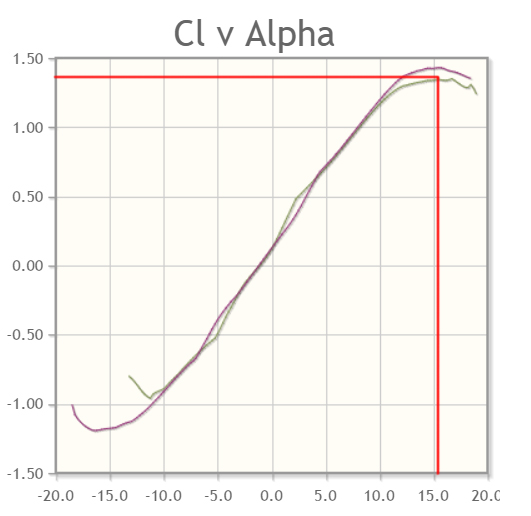
\includegraphics[width=.475\textwidth]{PerformanceAnalysis/Figures/clplot.jpg}
    \caption{Lift Coefficient Alpha Curve of The NACA 23015 Airfoil}
    \label{fig:NACA23015}
\end{figure}

The $C_{L}$ - $\alpha$ plot in \autoref{fig:NACA23015}\footnote{\url{http://airfoiltools.com/airfoil/details?airfoil=naca23015-il}, Accessed 24-05-2017} shows that for the Reynolds number of $3.0*10^{5}$, the $C_{L}$ will have a value of approximately 1.4. The two lines shown in the $C_{L}$ - $\alpha$ plot have Reynolds number of 200,000 and 500,000 each. 

\nomenclature[G]{$\alpha$}{Angle of Attack \nomunit{-}}


\subsection{Wing Loading}
An important parameter in the conceptual sizing of an aircraft is the wing loading. It is the ratio of the weight of the aircraft to the area of the reference wing \cite{aircraft_design}. It can be used to obtain a preliminary estimation of the wing surface area of each design providing a mass estimate is already made.
The driving flight condition for the sizing of the wing surface is when transitioning from the vertical to horizontal flight and vice versa. During this transition the UAV is required to fly at its stall speed which results in the lowest wing loading and hence the largest required wing surface area.

As explained in the previous chapter, the same airfoil is used during the trade-off for each design. In addition, the assumption is made that the stall speed of each design is  20 m/s. This speed was established by looking at reference UAVs and determining a rough ratio between maximum achievable speed and stall speeds. Analysis of different UAVs capable of flying at around 200 km/h has shown that this is a reasonable estimate. The stall speed is purposely chosen to be quite high, as importance is given to high speed flight which requires, as a general rule, less effective surface area. 

As the same airfoil is chosen and stall speed is set to be constant for all five concepts, from \autoref{eq:loading} it can be seen that the surface area, S, only varies with changes in the weight of the aircraft, W.

\begin{equation}
    \frac{W}{S}=\frac{1}{2} \cdot \rho \cdot V_{stall}^{2} \cdot C_{L_{max}}
    \label{eq:loading}
\end{equation}

Once the wing loading is calculated the surface area can be obtained by dividing the weights of the various concepts estimated in \autoref{sec:mass_esti} by the wing loading as shown in \autoref{eq:area}. The wingspan, b, and average chord, $\bar{c}$, can be calculated using \autoref{eq:wingspan} and \autoref{eq:chord} respectively and with the aspect ratios, A, presented in \autoref{sec:aspe_rati}. 

\nomenclature[B]{b}{Wing span \nomunit{m}}
\nomenclature[B]{$\bar{c}$}{Average chord \nomunit{m}}
\nomenclature[B]{A}{Aspect ratio \nomunit{-}}

\begin{minipage}{0.33\textwidth}
    \begin{equation}
        S = \frac{W}{\frac{W}{S}}
        \label{eq:area}
    \end{equation}
    \end{minipage}%
    \begin{minipage}{0.33\textwidth}
    \begin{equation}
        b =\sqrt{A \cdot S}
        \label{eq:wingspan}
    \end{equation}
    \end{minipage}%
    \begin{minipage}{0.33\textwidth}
    \begin{equation}
        \bar{c} = \frac{b}{A}
        \label{eq:chord}
    \end{equation}
\end{minipage}

The geometric properties of the wings of the five concepts are presented in \autoref{tab:wing_summ}.

\begin{table}[htb]
    \centering
    \caption{Table of Geometric Parameters of The Wings of The Five Concepts}
    \label{tab:wing_summ}
    \begin{tabularx}{\textwidth}{p{0.3\textwidth}p{0.2\textwidth}p{0.1\textwidth}p{0.15\textwidth}p{0.1\textwidth}}
        \toprule
        \textbf{Concept} & \textbf{W/S [kg/m$^2$]}  & \textbf{S [m$^2$]} & \textbf{b [m]} & \textbf{c [m]}\\\midrule
        The Tailsitter          &34.58                      & 1.50       & 2.60 & 0.58
        \\ \hdashline
        The Tandem              &34.58                      & 2.31       & 2.74 (ea.) & 0.42
        \\ \hdashline
        The Prandtl Box         &34.58                      & 1.88       & 2.57 & 0.37
        \\ \hdashline
        The Tiltrotor          &34.58                      & 2.17       & 3.45 & 0.63
        \\ \hdashline
        The Winged Quad.   &34.58                      & 1.27       & 3.19 & 0.40 \\\bottomrule
    \end{tabularx}
\end{table}

\nomenclature[B]{W/S}{Wing loading \nomunit{kg/m$^2$}}
\nomenclature[B]{S}{Wing surface area \nomunit{m$^2$}}

\section{Performance Criteria}
\label{sec:perf}

In this section, the different performance criteria used in the trade-off are analysed. From requirements \textbf{SYS-PF-1.3}, \textbf{SYS-PF-1.4} and \textbf{SYS-PF-2.3}, it has been deduced that the most important parameters regarding performance are the range, the endurance and the required power for the UAV. Other performance specific properties like drag and mass are included in these calculations.  
First, the endurance analysis is presented in \autoref{sec:endu_ana}\begin{comment}No autoref on purpose here \end{comment}%
. Then, in \autoref{sec:range_ana}\begin{comment}No autoref on purpose here \end{comment}%
, a preliminary range difference between the different concepts in calculated and finally, in \autoref{sec:power_ana}\begin{comment}No autoref on purpose here \end{comment}%
, the required power for different cases is obtained.

\subsection{Endurance Analysis}
\label{sec:endu_ana}

In this section, the maximum endurance of each concept is analysed. It is assumed that the drone is flying at an optimal flight condition for maximum endurance. Neither take-off and landing nor any other flight condition are included in the calculations of this analysis.

To calculate the maximum endurance of each concept, the optimum lift coefficient of each concept has to be calculated. This is achieved using \autoref{eq:lift_end}, derived by minimising the required power.

\begin{equation}
    C_{L_{endu}} = \sqrt{\frac{3\cdot C_{D_0}}{k}} \quad \mathrm{where} \quad k=\frac{1}{\pi \cdot e\cdot A}
    \label{eq:lift_end}
\end{equation}

Then setting the weight equal to the lift gives the optimum velocity for maximum endurance flight.

\begin{equation}
    V_{opt} = \sqrt{\frac{2\cdot W}{\rho\cdot S\cdot C_{L_{opt}}}}
    \label{eq:vopt}
\end{equation}

The maximum endurance is then obtained using \autoref{eq:endurance} \cite{ran_end}.

\begin{equation}
    E = (R\cdot t)^{1-n}\cdot \Bigg{[}\frac{\eta_{tot}\cdot U\cdot C}{\frac{1}{2}\cdot\rho \cdot V_{opt}^3\cdot S\cdot C_{D_0} + \frac{2\cdot W^2\cdot k}{\rho\cdot V_{opt}\cdot S}}\Bigg{]}^n
    \label{eq:endurance}
\end{equation}

For further analysis, efficiency factors are assumed to be equal to one. This means $\eta_{tot}=1$, $(R\cdot t)=1$ and $n=1$. Then, as the energy $U\cdot C$ depends on the type and mass of energy source, a preliminary energy estimation can to be done for the performance calculation. As a first order estimation it is assumed that the battery used is of the Lithium-Ion type, having an average energy density of 135 $\frac{W\cdot h}{kg}$. They are used for their high energy density compared to other available battery types. Disadvantages however are a higher cost and the need of a robust protection to ensure reliability. Using a preliminary battery mass estimation of 2 kg, an energy of 270 $W\cdot h$. Care should be taken to not confuse the estimated values of the endurance with the actual endurance the design can achieve. Although acceptable assumptions have been made for all of the variables, it is not possible yet to accurately obtain the properties at this stage of the design process. Furthermore, required amount of energy and hence battery mass depends on each design. In order to perform a fair trade-off, each design is assumed to have the same battery mass. Because the same methods have been applied for the generation of all the variables, the relative difference between the endurance values is still acceptable and can thus be used for the trade-off. \autoref{tab:trade_endu} gives a general overview of the endurance of each concept. The endurance is expressed in hours and in a percentage. The percentage value is the percentage of the endurance of the concept with respect to the average of all the concepts, as explained in \autoref{sec:grading_sys_perf}.

\begin{equation}
    E =  \frac{U\cdot C}{\frac{1}{2}\cdot \rho\cdot V_{opt}^3\cdot S\cdot C_{D_0} + \frac{2\cdot W^2\cdot k}{\rho \cdot V_{opt}\cdot S}}
    \label{eq:endurance_simpl}
\end{equation}

\begin{table}[htb]
    \centering
    \caption{Overview of Endurance Ranking for Each Concept}
    \label{tab:trade_endu}
    \begin{adjustbox}{width=1\textwidth}
    \small
        \begin{tabular}{lcccc}
        \toprule
        \textbf{Concept} & \textbf{Weight [N]} & \textbf{Aspect Ratio [-]} & \textbf{V$_{Endurance}$ [m/s] }& \textbf{Endurance [\%], [hrs]} \\ \midrule
        The Tailsitter          &540   &4.5 &24  & 78, 0.23\\\hdashline
        The Tandem              &569   &6.5 & 17 & 82, 0.24\\\hdashline
        The Prandtl Box         &373   &7  & 14& 168, 0.50\\\hdashline
        The Tiltrotor           &647   &5.5   & 20 & 60, 0.18\\\hdashline
        The Winged Quad.        &431   &8   &20 & 112, 0.33\\\bottomrule
        \end{tabular}
        \end{adjustbox}
\end{table}



\subsection{Range Analysis}
\label{sec:range_ana}
In this section, the range of each concept is calculated. For this, it is assumed that the drone is performing a simple mission of only trying to achieve maximum distance. Neither take-off \& landing nor any other mission related phase are included in these calculations. 

The range analysis is performed similarly to the endurance analysis. The only difference lies in the flight condition for maximum range. The lift coefficient is approximated using \autoref{eq:lift_ran}, derived by maximising the lift over drag ratio. 

\begin{equation}
    C_{L_{range}} = \sqrt{\frac{C_{D_0}}{k}} \quad where \quad k=\frac{1}{\pi\cdot e\cdot A}
    \label{eq:lift_ran}
\end{equation}

The optimal velocity for maximum range can again be calculated using \autoref{eq:vopt}. Then the endurance at maximum range conditions is obtained using \autoref{eq:endurance_simpl} and finally using \autoref{eq:range} the range is calculated.

\begin{equation}
    R = E\cdot V_{range}
    \label{eq:range}
\end{equation}

In \autoref{tab:trade_range} the range for each of the concepts is shown. The trade-off ranking can also be seen for each concept. As with the endurance ranking, the absolute values in the Table of low accuracy and they will thus only be used for the ranking of the designs due to their relative difference. 

\begin{table}[H]
    \centering
    \caption{Overview of Range Ranking for Each Concept}
    \label{tab:trade_range}
    \begin{adjustbox}{width=1\textwidth}
    \small
        \begin{tabular}{lcccc}
        \toprule
        \textbf{Concept} & \textbf{Weight [N]} & \textbf{Aspect Ratio [-]} & \textbf{V$_{range}$ [m/s] } &\textbf{Range [\%],[km]}  \\ \midrule
        The Tailsitter           &540 &4.5& 32  & 104, 23\\\hdashline
        The Tandem               &569 &6.5& 22   & 77, 17\\\hdashline
        The Prandtl Box          &373 &7 & 18 & 129, 29\\\hdashline
        The Tiltrotor            &647 &5.5  &27 & 68, 15\\\hdashline
        The Winged Quad.         &431 &8  &25.7 &123, 27 \\\bottomrule
        \end{tabular}
        \end{adjustbox}
\end{table}


\subsection{Power Analysis}
\label{sec:power_ana}

In order to assess whether each of the five concepts can meet the challenging requirements derived from the various stakeholder needs, an analysis on the power required for the various flight phases is necessary. The power required to hover and climb vertically will therefore be calculated for the five concepts and compared. Later on the power required for climb during the horizontal flight phase will be calculated.


\subsubsection{Vertical Flight Phase}
During vertical flight the engines/rotors needs to overcome the weight of the UAV, i.e. the thrust to weight ratio must be greater than one ($\frac{T}{W} \ge 1$). The required power for both hovering and vertical climb will therefore be analysed.

\subsubsection*{Power Required to Hover}
During hovering, since the vertical velocity is zero, thrust is generated by accelerating air from zero velocity from all directions through the rotor disk. Employing the conservation of both energy and momentum, the power required to hover can be expressed as a function of weight and is characterised by \autoref{eq:powe_requ_hove} below\footnote{\url{http://s6.aeromech.usyd.edu.au/aerodynamics/index.php/sample-page/aircraft-performance/hoverclimbdescent-analysis/}, Accessed 18-05-2017}.

\begin{equation}
\label{eq:powe_requ_hove}
\begin{split}
  P_{req} &= W \cdot v_{\imath} \qquad \mathrm{where,} \quad v_{\imath} = \sqrt{\frac{(T = W)}{2 \cdot \rho \cdot A}}\\
\Rightarrow  P_{req} &= \sqrt{\frac{W^3}{2 \cdot \rho \cdot A}}
\end{split}
\end{equation}

\nomenclature[B]{$P_{req}$}{Power required \nomunit{kW}}
\nomenclature[B]{$W$}{Weight \nomunit{N}}
\nomenclature[B]{$v_{\imath}$}{Induced velocity at rotor disk \nomunit{m/s}}

The power required to hover is therefore proportional to the square root of weight cubed, i.e. $P \propto W^{\frac{3}{2}}$ and it is therefore clear that the lighter the UAV is, the less power is required to hover. The concepts are therefore ranked from lowest to highest required power.

\subsubsection*{Power Required to Climb}

During a vertical climb at a constant velocity the air flow through the rotor already has momentum. This changes the required power to maintain such a climb as the induced velocity is now different. The power required for vertical climbing flight is given by \autoref{eq:powe_requ_clim}. It is important to note that if the climb rates are small, thrust and weight can be considered equal (i.e. $T = W$).

\begin{equation}
\label{eq:powe_requ_clim}
\begin{split}
  P_{req} &= W \cdot v_{\imath} \qquad \mathrm{where,} \quad v_{\imath} = \frac{V_{c}}{2} + \sqrt{ \left( \frac{V_{c}}{2} \right) ^2 + \frac{(T = W)}{2 \rho A}}\\
  \Rightarrow P_{req} &= W \left( \frac{V_{c}}{2} + \sqrt{ \left( \frac{V_{c}}{2} \right) ^2 + \frac{W}{2 \rho A}} \right)
\end{split}
\end{equation}

As the vertical climb rate is set to a constant value of 4 m/s as stipulated by requirement \textbf{SYS-PF-2.4} it is clear that the required power increases with increasing weight. As can be seen in \autoref{eq:powe_requ_clim} the drag is not included.This if for two reasons, firstly preliminary calculations show that they are in the order of 10 N for the prescribed climb rate and secondly the goal of this analysis is primarily to determine how much power each concept requires relative to the others.

\subsubsection{Disk Loading}

In order to evaluate the power equations presented above (namely Equations \ref{eq:powe_requ_hove} \& \ref{eq:powe_requ_clim}) the area of the rotor disk, A is required. By obtaining a value for the disk loading, (W/A) of the five concepts coupled with knowing the mass estimate of each concept, the rotor disk area can be calculated ($A = \frac{W}{(W/A)}$).

From the graph presented in \autoref{fig:MTOW_vs_disk_load} a relationship was established between the MTOW and the disk loading.

\begin{figure}[H]
\centering
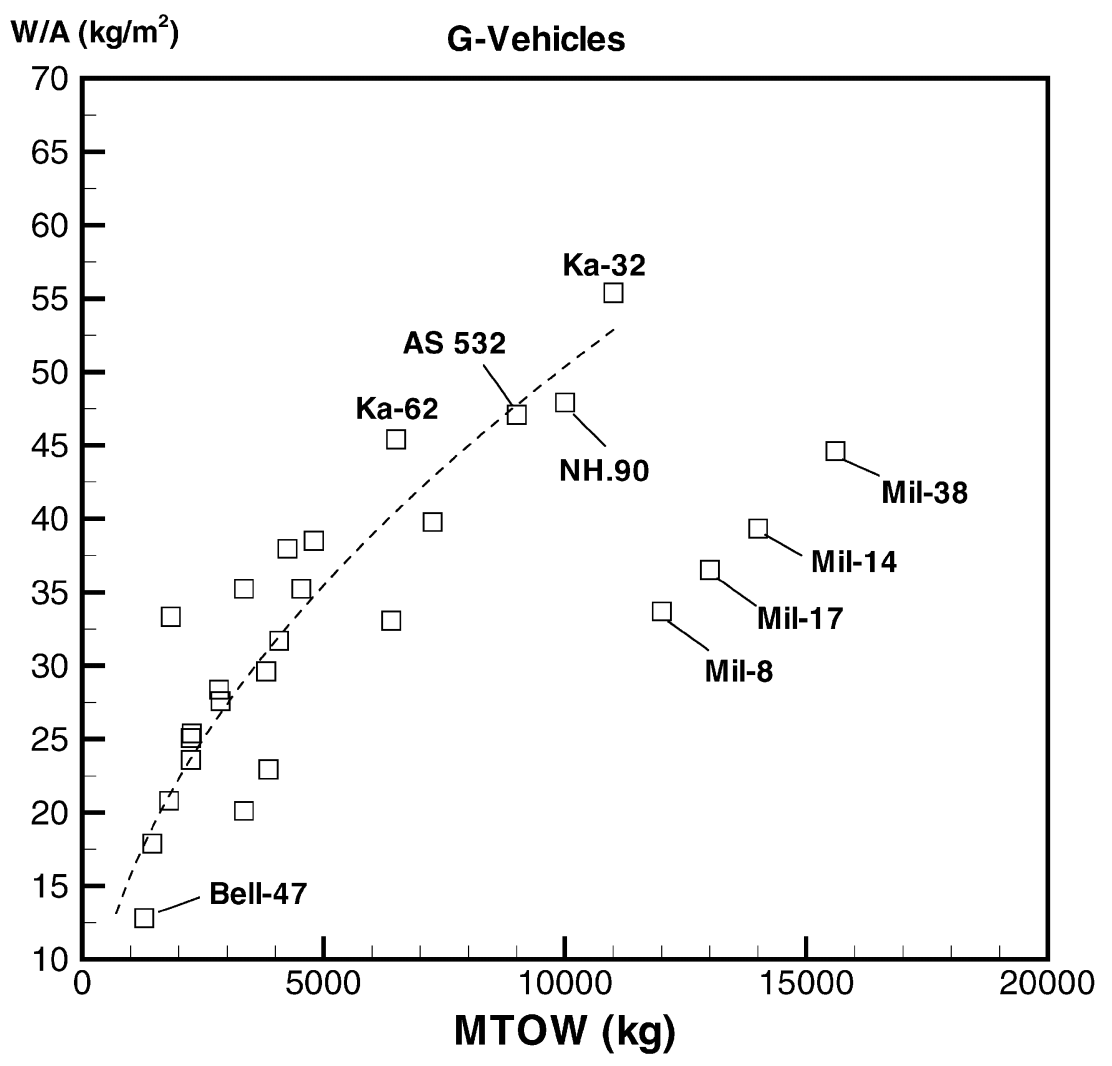
\includegraphics[width=0.75\textwidth]{PerformanceAnalysis/Figures/DiskLoading_vs_MTOW.png}
\caption{Graph of Disk Loading Versus MTOW \cite{diskloading}}
\label{fig:MTOW_vs_disk_load}
\end{figure}

The disk loading can be approximated as a linear function of MTOW and is expressed as in \autoref{eq:disk_load}. 

\begin{equation}
\label{eq:disk_load}
(W/A) = 0.0031 \cdot MTOW + 15.03
\end{equation}



\subsubsection{Power Required for Maximum Velocity}

The maximum power required during horizontal flight is achieved at maximum velocity, that is at 200 km/h (55.6 m/s) as stipulated by requirement \textbf{SYS-PF-1.2}. The power required is defined by \autoref{eq:PR}.

\begin{equation}
    P_{r} = C_D\cdot \frac{1}{2}\cdot\rho \cdot V^3\cdot S
    \label{eq:PR}
\end{equation}

The drag coefficient is calculated in \autoref{eq:cd}, where the zero lift drag coefficient is obtained in \autoref{sec:zeroliftdrag} and the lift coefficient is calculated using \autoref{eq:liftcoef}. 

\begin{equation}
    C_L = \frac{2\cdot W}{\rho \cdot V^2\cdot S}
    \label{eq:liftcoef}
\end{equation}

\begin{equation}
    C_D = C_{D_0} + \frac{C_L^2}{\pi \cdot e\cdot A}
    \label{eq:cd}
\end{equation}

The results for each concept are summarised in \autoref{tab:powe_requ_hove}.

\subsubsection{Summary}

Having established the calculation for the power required in the three most important cases, namely maximum velocity, hovering and climbing, the concepts can be ranked for the trade-off. \autoref{tab:powe_requ_hove} illustrates each concept and their different required powers. Then, the maximum of these values is used for the trade-off. As for each concept this value will drive the design of the propulsion subsystem. The maximum P$_{req}$ is also given as a percentage value with respect to the average of all the maxima.

\begin{table}[H]
\centering
\caption{Table Ranking Concepts Based On Power Required}
\label{tab:powe_requ_hove}
\begin{tabular}{p{3.5cm} >{\centering}p{2.6cm} >{\centering}p{2.6cm} p{2.6cm}<{\centering} p{2.4cm}<{\centering}}
\toprule
 \textbf{Concept}  & \textbf{P$_{req}$ for max velocity [kW]}    & \textbf{P$_{req}$ to hover [kW]}  & \textbf{P$_{req}$ to climb [kW]} & \textbf{Max P$_{req}$ [\%],[kW]}
\\ \midrule
 The Tailsitter    &        2.8                     &  4.2                   & 5.5   &  74,5.5 \\ \hdashline
 The Tandem        &        10.2                   &  5.0                   & 6.4   & 136,10.2 \\\hdashline
 The Prandtl-Box   &        9.0                   &  2.9                    &3.8  & 120,9.0\\ \hdashline
 The Tiltrotor     &              8.0                &  5.1                   & 6.4  & 107,8.0 \\ \hdashline
 The Winged Quad.  &                  4.7            &  3.4                    &4.4  & 63,4.7 \\ \bottomrule
\end{tabular}
\end{table}






